\subsection{Внутреннее проектирование}
\subsubsection{Разработка структуры системы}

Подсистема предназначена для включения в крупные системы. В частности в подсистеме не решается вопрос сбора и первичной обработки новостных данных -- это берёт на себя система верхнего уровня.

Разрабатываемая подсистема состоит из двух функциональных модулей.

Структура подсистемы показана в графической части дипломного проекта на листе «Структурная схема».

\paragraph{Анализ информационных потоков} \hfill

Анализ предметной области определил два источника информации:

\begin{itemize}
\item ИПС -- предоставляет API доступа и редактирования к актуальной базе новостей
\item Эксперт -- создаёт/редактирует запросы, редактирует контура стран/провинций
\end{itemize}

Получение информации от ИПС происходит посредством http запросов. Для обмена информацией используется стандарт формата JSON.

Создание и редактирование запросов экспертом происходит посредством специализированного клиентского приложения.

Создание и редактирование контуров стран/провинций происходит с помощью специализированного ПО, которое не входит в состав разрабатываемой подсистемы.

\clearpage
\paragraph{Определение состава компонентов системы} \hfill

Согласно требованиям ТЗ касательно функциональности разрабатываемой подсистемы, можно выделить следующие составляющие компоненты.

\subparagraph{Модуль геотегирования.} \hfill

Должен обеспечивать процесс геотегирования по следующей методике:

\begin{enumerate}
\item циклично выполняются все сохранённые в базе запросы на ИПС
\item для документов не имеющих геометку ставится геометку соответствующего запроса.
\end{enumerate}

Должен предоставлять пользователю эксперту интерфейс для создания и редактирования тегирующих запросов до странам/провинциям.

Входные данные:
\begin{itemize}
\item Действия над запросами: добавление, удаление, обновление;
\item Сохранённые запросы
\item Результаты выполнения сохранённых запросов на ИПС
\end{itemize}

Выходные данные:
\begin{itemize}
\item Сохранённые запросы
\item Изменение новостей
\end{itemize}

\clearpage
\subparagraph{Модуль прогнозирования.} \hfill

Должен анализировать по провинциям частоты основных тем по дням рассмативаемого периода и предсказывать частоту упоминания основных тем новостей.

\begin{itemize}
\item График количества документов, соответствующих сохранённому запросу, используемого для прогнозирования, по дням до текущей даты;
\item График прогнозируемого количества документов, соответствующих сохранённому запросу, используемого для прогнозирования, по дням на всём рассматриваемом интервале времени;
\item Аналитическую формулу прогноза, по которой значение количества документов, соответствующих сохранённому запросу, можно вычислить для любого дня рассматриваемого интервала времени;
\item Количественную оценку полученного прогноза;
\end{itemize}

Входные данные:
\begin{itemize}
\item параметры эволюционного алгоритма 
\item параметры метода скользящего среднего
\item параметры полиноминальной регрессии
\item веса методик
\item сохраненный формализованный запрос для прогнозирования.
\end{itemize}

Выходные данные:
\begin{itemize}
\item прогноз частоты тем по провинциям
\end{itemize}

\clearpage
\subparagraph{Модуль клиентского приложения.} \hfill

Должен предоставлять пользователю полную информацию о документе (новости) и его реквизитах. Также модуль должен предоставлять возможность редактировать реквизиты документа (за исключением идентификатора и источника) и возможность удаления новости из АИС.

Реквизиты документа:
\begin{itemize}
\item Заголовок новости -- краткий заголовок новости;
\item Основная часть новости -- основной массив текста с форматированием;
\item Время публикации новости -- время публикации новости, указанное в
источнике;
\item Рубрика новости -- категория новости, к которой она относится;
\item Источник новости -- адрес сайта новости;
\item Идентификатор новости -- уникальный идентификатор новости, под
которым она хранится в БД.
\item Метки новости -- список строк-меток, которые были присвоены новости;
\end{itemize}

Входные данные:
\begin{itemize}
\item Запрос на проблемно-ориентированном языке для подсветки основной части документа. Может отсутствовать, тогда отображается весь текст документа без подсветки.
\item Идентификатор документа для отображения.
\item Обновленные значения реквизитов документа при их редактировании.
\end{itemize}

Выходные данные:
\begin{itemize}
\item Реквизиты документа, перечисленные выше.
\item Обновлённые данные в базе данных и индексе при редактировании полей документа.
\end{itemize}


\subparagraph{Структура модулей подсистемы.} \hfill

Структура модулей представлена в графической части на листе <<Структура подсистемы>>

Помимо вышеописанных модулей, так же в проекте планируются подмодули настроек модулей.

\begin{figure}[!h]
\centering
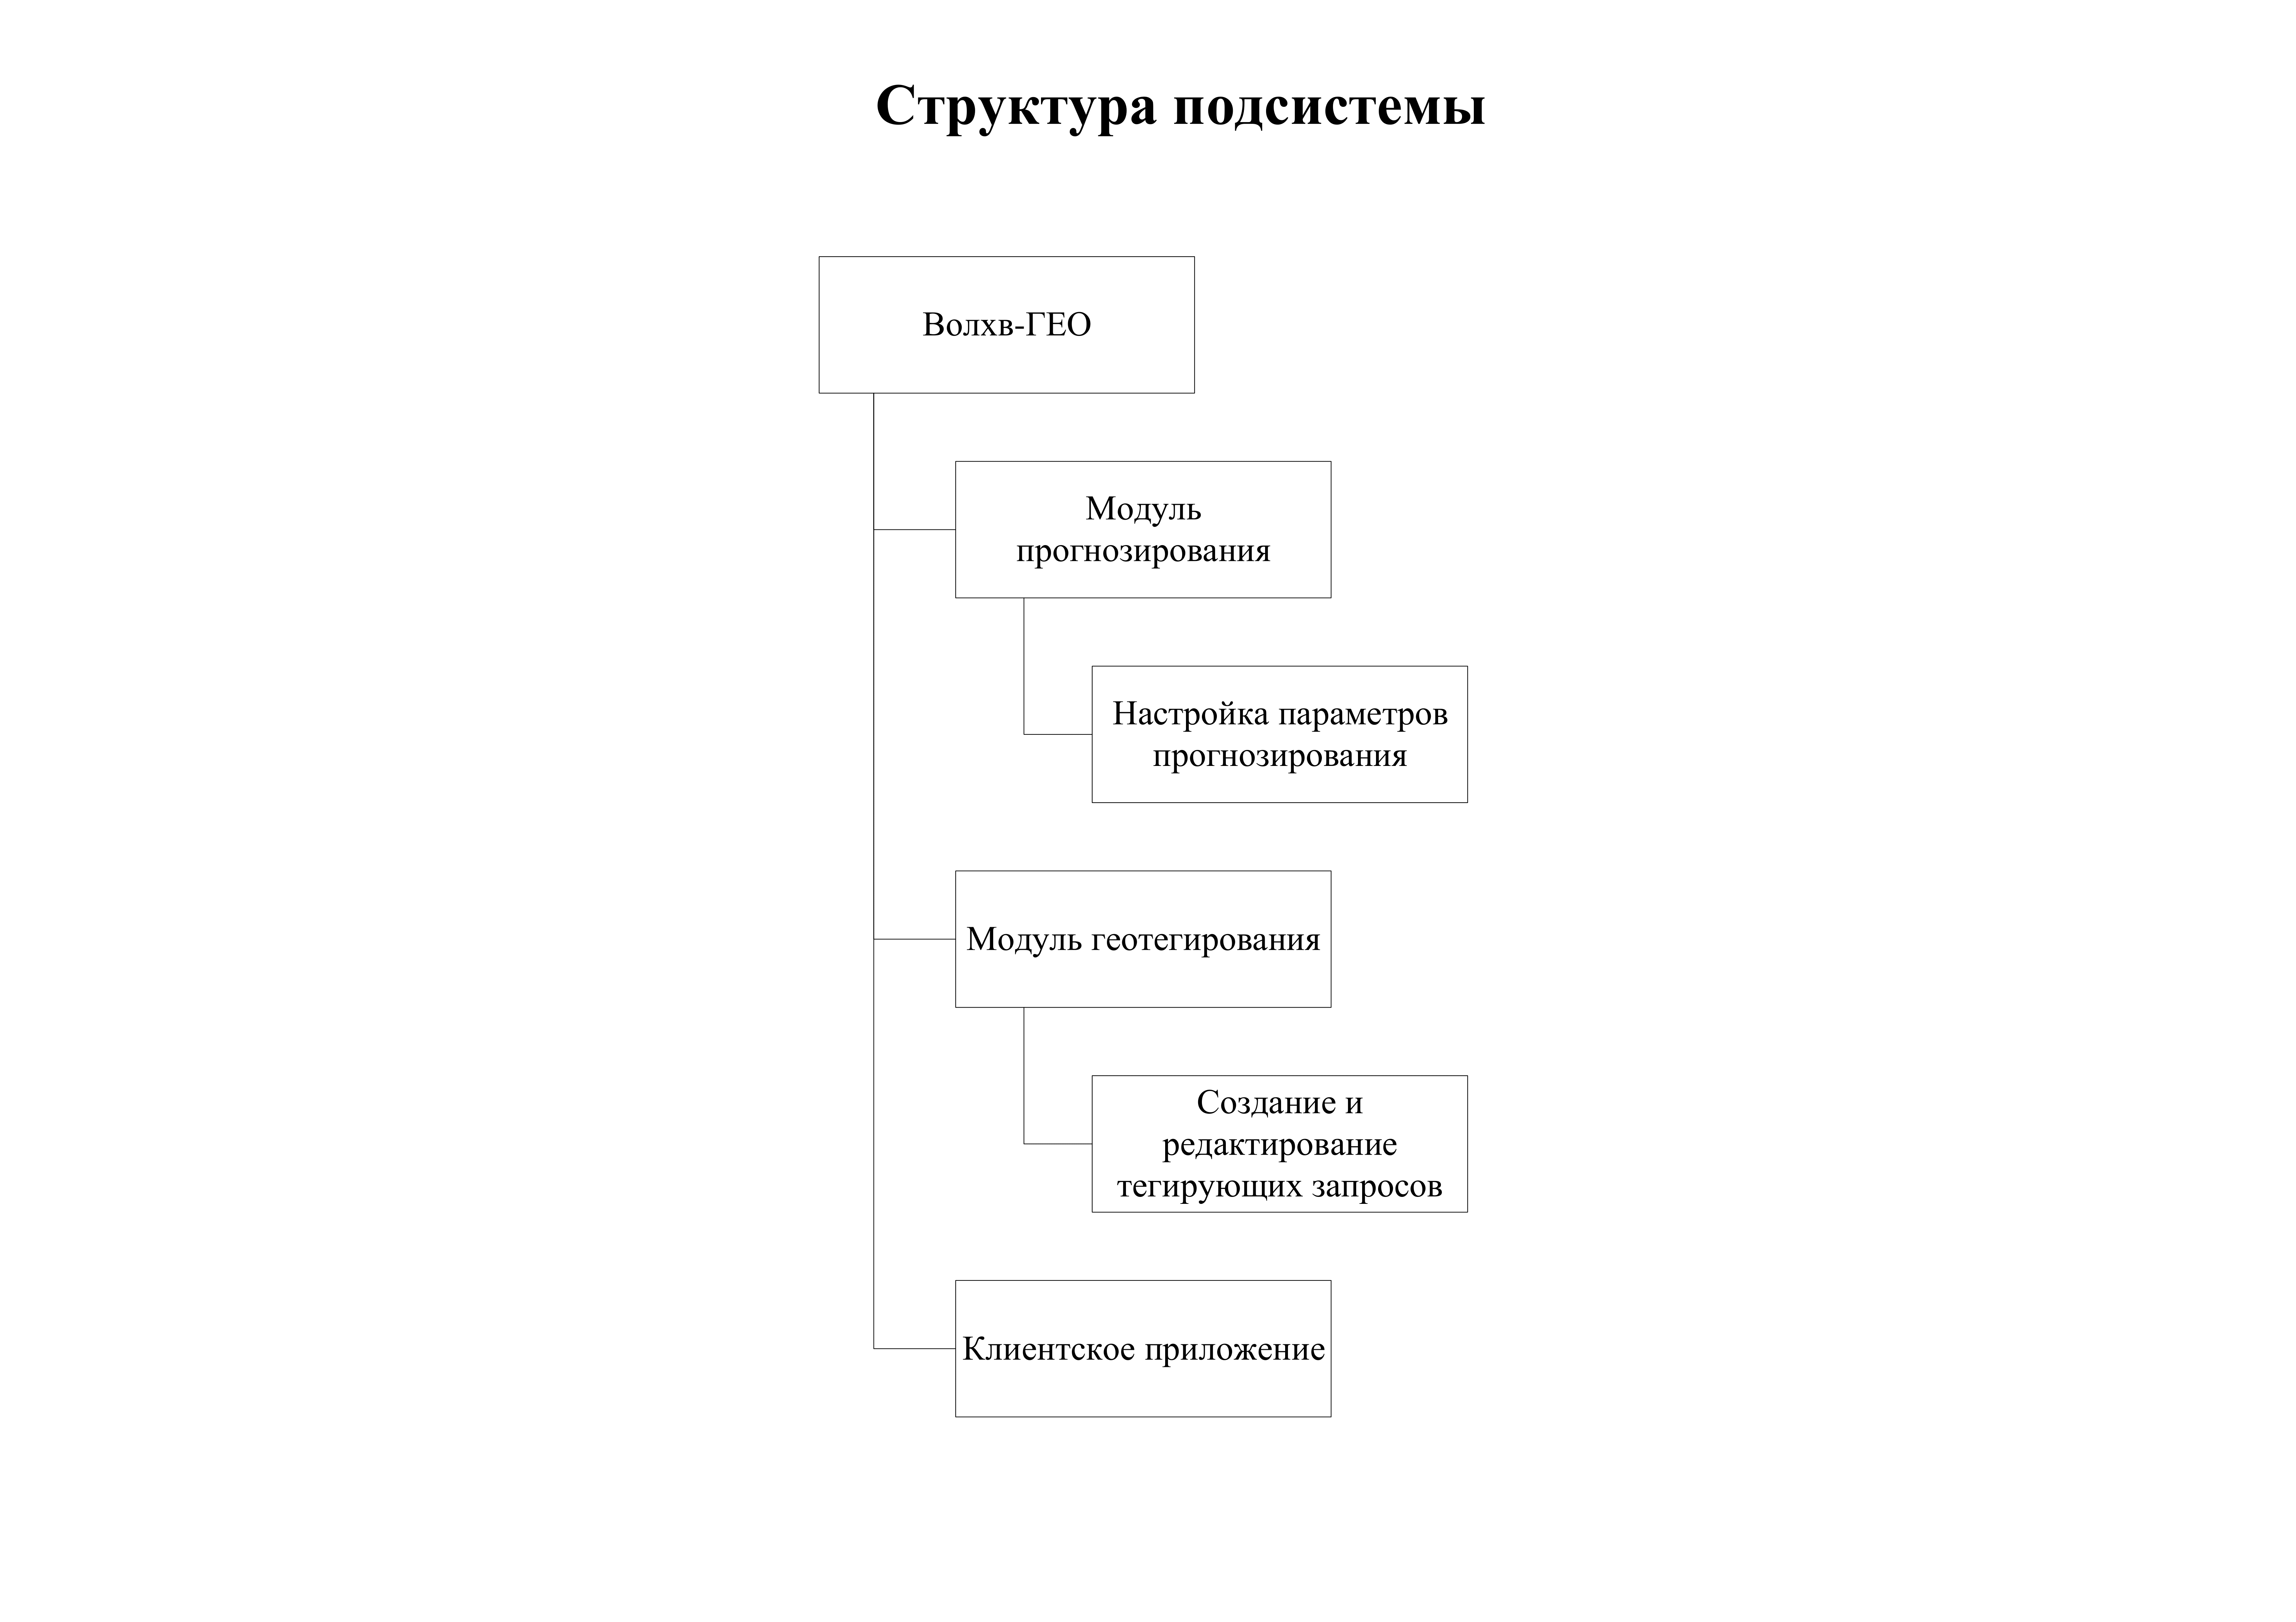
\includegraphics[width=\textwidth]{design/ramkaless/6.png}
\label{figure:structPodsis}
\caption{Структура подсистемы.}
\end{figure}